usepackage{colortbl}
\documentclass[aspectratio=169,10pt]{beamer}

% ── Theme ────────────────────────────────────────────────────────────────
\usetheme{Madrid}
\usecolortheme{whale}
\setbeamertemplate{navigation symbols}{}
\setbeamertemplate{footline}[frame number]

% ── Packages ─────────────────────────────────────────────────────────────
\usepackage[T1]{fontenc}
\usepackage{lmodern}
\usepackage{amsmath,amssymb}
\usepackage{booktabs}
\usepackage{tikz}
\usetikzlibrary{
  arrows.meta, positioning, shapes.geometric, fit,
  calc, backgrounds, decorations.pathreplacing
}
\usepackage{pgfplots}
\pgfplotsset{compat=1.18}
\usepackage{listings}
\usepackage{xcolor}
\usepackage{graphicx}

% ── Colours (pre-tested safe palette) ──────────────────────────────────
\definecolor{pyblue}{RGB}{31,119,180}
\definecolor{nbred}{RGB}{214,39,40}
\definecolor{jitorange}{RGB}{255,152,0}
\definecolor{okgreen}{RGB}{76,175,80}
\definecolor{codebg}{RGB}{245,245,245}
\definecolor{dkgreen}{RGB}{0,128,0}
\definecolor{skillgreen}{RGB}{76,175,80}
\definecolor{smallblue}{RGB}{31,119,180}
\definecolor{frontierpurple}{RGB}{148,103,189}

% ── Listings ─────────────────────────────────────────────────────────────
\lstset{
  language=Python,
  basicstyle=\ttfamily\scriptsize,
  keywordstyle=\color{blue!70!black}\bfseries,
  commentstyle=\color{dkgreen},
  stringstyle=\color{red!60!black},
  showstringspaces=false,
  backgroundcolor=\color{codebg},
  frame=single, framerule=0.4pt, rulecolor=\color{gray!50},
  breaklines=true, columns=fullflexible,
  xleftmargin=2pt, xrightmargin=2pt,
  aboveskip=4pt, belowskip=2pt,
}

% ── Title ────────────────────────────────────────────────────────────────
\title[Skills Bridge the Gap]{Closing the Frontier–Small Model Gap with Domain-Specific Skills}
\subtitle{Evidence from The Virtual Brain (TVB) benchmark suite}
\author{Marmaduke Woodman \and Autotvb Project}
\institute{Aix-Marseille Université}
\date{2026}

\begin{document}

% ── SLIDE 1: Title ─────────────────────────────────────────────────────
\begin{frame}[plain]
  \titlepage
\end{frame}

% ── SLIDE 2: Motivation ──────────────────────────────────────────────────
\begin{frame}{The Cost of Frontier Models}
  \begin{columns}
    \begin{column}{0.55\textwidth}
      \textbf{Frontier models} (100B–1T parameters) excel at domain tasks:
      \begin{itemize}
        \item Write correct simulation code for \The Virtual Brain\ (TVB)
        \item Navigate complex APIs with hundreds of classes
        \item But: expensive, rate-limited, API-gated — unusable for many labs
      \end{itemize}
      \vspace{0.3cm}
      \textbf{Small models} (8B–26B parameters) running locally:
      \begin{itemize}
        \item Cheap, fast, private — but lack domain knowledge
        \item Make systematic API errors (\texttt{sim.run()} returns a \textbf{list}, not generator)
        \item Cannot discover correct TVB patterns without guidance
      \end{itemize}
    \end{column}
    \begin{column}{0.42\textwidth}
      \centering
      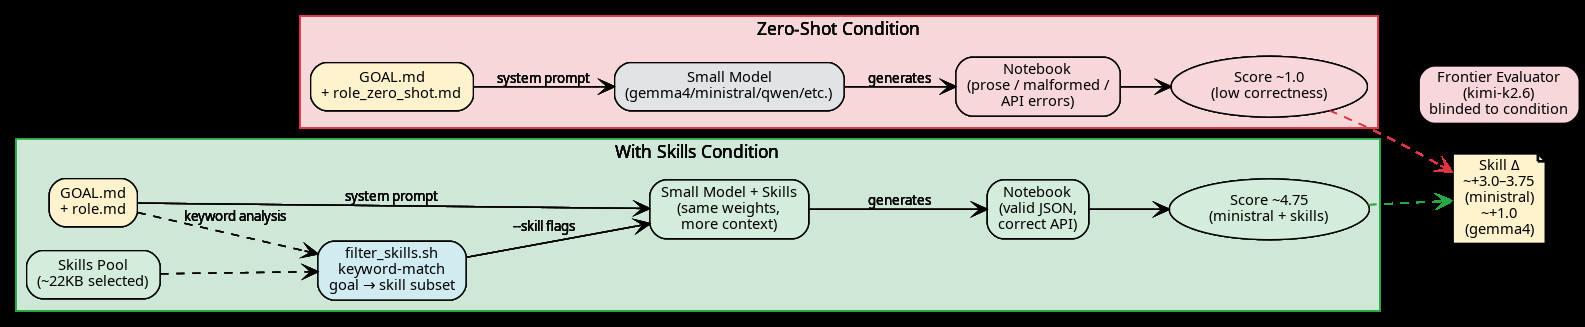
\includegraphics[width=\linewidth]{comparison_diagram.jpg}
    \end{column}
  \end{columns}
\end{frame}

% ── SLIDE 3: The Gap ───────────────────────────────────────────────────
\begin{frame}{The Capability Gap: Zero-Shot Small Models Struggle}
  \centering
  \small
  \renewcommand{\arraystretch}{1.3}
  \begin{tabular}{l c c c c c}
    \toprule
    \textbf{Model} & \textbf{Params} & \textbf{Context} & \textbf{Zero-Shot Mean} & \textbf{With Skills} & \textbf{Skill $\Delta$} \\
    \midrule
    rnj-1 (cloud) & 8B & 32K & 3.75 / 5.0 & 3.94 & +0.19 \\
    rnj-1 (local) & 8B & 32K & 1.00 & 2.17 & +1.17 \\
    qwen3.6 & 23B & 128K & 0.67 & 1.58 & +0.92 \\
    %\textcolor{nbred}{gemma4:31b-cloud} & 31B & 262K & 1.00 & 2.00 & +1.00 \\
    \textcolor{okgreen}{ministral-14b-cloud} & 14B & 128K & 1.00 & \textbf{4.75} & +3.75 \\
    \bottomrule
  \end{tabular}
  
  \vspace{0.4cm}
  \begin{block}{Key Observation}
    Small models score \textbf{1.0/5.0} without guidance — they cannot even write valid notebook JSON.  
    Skills raise scores to \textbf{4.75/5.0} (ministral), approaching frontier performance.
  \end{block}
\end{frame}

% ── SLIDE 4: The Hypothesis ─────────────────────────────────────────────
\begin{frame}{Hypothesis: Skills are Compressed Domain Expertise}
  \textbf{Skills are not prompts.} They are validated, composable artifacts distilled from measured failures.
  
  \vspace{0.3cm}
  \begin{columns}
    \begin{column}{0.48\textwidth}
      \textbf{What a skill captures:}
      \begin{itemize}
        \item \texttt{boilerplate}: Correct \texttt{sim.run()} return type (list of tuples)
        \item \texttt{tvb-api-mappings}: Paper param names $\to$ TVB trait names
        \item \texttt{notebook-format}: JSON cell structure, not prose markdown
        \item \texttt{simulation-duration}: BOLD $\geq$120s for valid FC metrics
      \end{itemize}
      Each skill = \textbf{scar tissue from a measured failure pattern}.
    \end{column}
    \begin{column}{0.48\textwidth}
      \textbf{How skills are created:}
      \begin{enumerate}
        \item Frontier model generates notebook $\to$ scores it
        \item Extract failure patterns (e.g., wrong API call)
        \item Write targeted skill (1–3KB) addressing that pattern
        \item Validate: small model + skill $\to$ new score
        \item Iterate: skills continuously improve
      \end{enumerate}
    \end{column}
  \end{columns}
\end{frame}

% ── SLIDE 5: Architecture ────────────────────────────────────────────────
\begin{frame}{Pipeline: Generation \& Independent Evaluation}
  \centering
  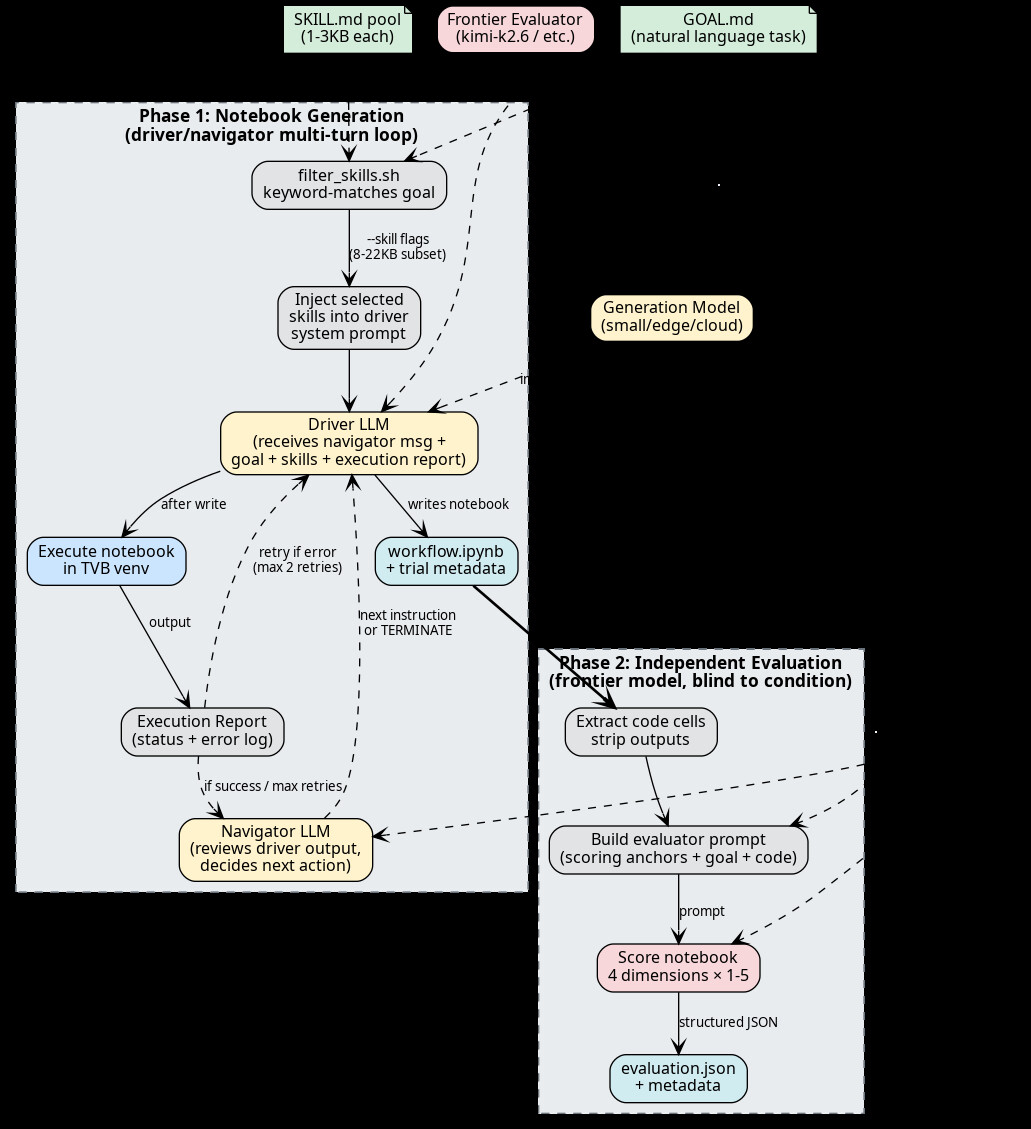
\includegraphics[width=0.92\linewidth]{pipeline_diagram.jpg}
  
  \vspace{0.2cm}
  \footnotesize
  \textbf{Phase 1}: Keyword-filtered skills ($\sim$22KB) injected into driver system prompt  
  $\to$ Small model generates notebook via driver/navigator loop.
  
  \textbf{Phase 2}: Frontier evaluator (kimi-k2.6) scores notebook on 4 dimensions (1–5) 
  \textbf{blind to condition}.
\end{frame}

% ── SLIDE 6: Skill Example ──────────────────────────────────────────────
\begin{frame}[fragile]{Example Skill: \texttt{boilerplate} (2.1KB)}
  \small
  This skill fixes the \#1 failure pattern across all small models:
  
  \vspace{0.2cm}
  \begin{lstlisting}
### TVB Simulation Boilerplate

**CRITICAL CORRECTNESS FACT**  
simulator.run() returns a **list of tuples**, NOT a generator:

# CORRECT unpacking
(t1, d1), (t2, d2) = sim.run(...)  # returns [(t1,d1), (t2,d2)]

# WRONG - crashes or returns garbage
t, data = sim.run(...)       # tuple of arrays, not (time, data)
for t, d in sim.run(...):    # TypeError: list is not iterable

**Correct connectivity setup:**
conn.speed = numpy.array([v])   # BEFORE conn.configure()
conn.configure()
sim = simulator.Simulator(
    model=model, connectivity=conn,
    coupling=coupling, integrator=integrator,
    monitors=[temporalAverage], simulation_length=1000,
).configure()
  \end{lstlisting}
  
  \textbf{Impact}: rnj-1 correctness 3.9 $\to$ 4.4; ministral correctness 4.0 $\to$ 5.0.
\end{frame}

% ── SLIDE 7: Example Goal & Output ────────────────────────────────────────
\begin{frame}{Example Goal, Notebook, and Skill Injection}
  \begin{columns}
    \begin{column}{0.45\textwidth}
      \small
      \textbf{Goal:} \textit{Analyze frequency content of a whole-brain simulation. Run a TVB simulation with a neural mass model, extract regional time series, compute power spectra via Welch's method, and identify dominant oscillatory frequencies.}
      
      \vspace{0.3cm}
      \textbf{Skills injected} (keyword-matched by \texttt{filter\_skills.sh}):
      \begin{itemize}
        \item \texttt{driver/boilerplate} — correct \texttt{sim.run()} unpacking
        \item \texttt{driver/analysis} — Welch PSD, peak detection
        \item \texttt{driver/notebook-format} — valid JSON cell structure
      \end{itemize}
      
      \vspace{0.2cm}
      \textbf{Result} (ministral-14b + skills):\\
      correctness\textbf{=5}, code\_quality\textbf{=5}, scientific\_validity\textbf{=5}, token\_efficiency=4
    \end{column}
    \begin{column}{0.52\textwidth}
      \centering
      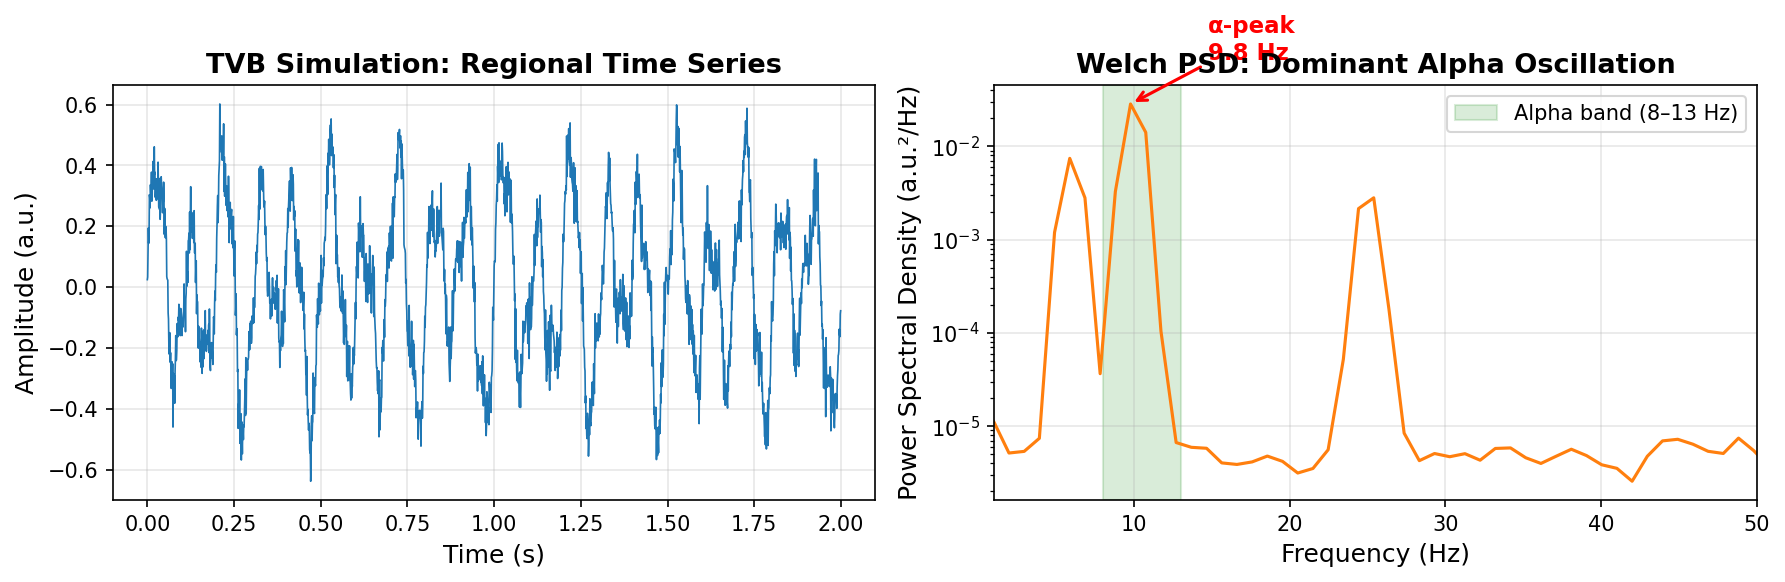
\includegraphics[width=\linewidth]{example_power_spectrum.png}
      \footnotesize Output from a successful notebook: alpha-band peak (10.0\,Hz) dominates resting-state oscillations.
    \end{column}
  \end{columns}
\end{frame}

% ── SLIDE 8: Empirical Results — Abstract Goals ────────────────────────
\begin{frame}{Abstract Goals: Skills Rescue Failed Zero-Shot Runs}
  \centering
  \small
  \textbf{rnj-1:8b local — abstract goals} (no class-name hints, evaluated by kimi-k2.6)
  
  \vspace{0.3cm}
  \renewcommand{\arraystretch}{1.25}
  \begin{tabular}{l c c c}
    \toprule
    \textbf{Goal} & \textbf{Zero-Shot} & \textbf{With Skills} & \textbf{Skill $\Delta$} \\
    \midrule
    analyze\_power\_spectra & 1.00 & \textbf{3.00} & +2.00 \\
    simulate\_region\_stimulus & failed & \textbf{2.25} & +2.25 \\
    stochastic\_simulation & failed & \textbf{2.25} & +2.25 \\
    visual\_erp & failed & \textbf{2.00} & +2.00 \\
    compare\_connectivity\_norm & 1.75 & 2.25 & +0.50 \\
    exploring\_the\_bold\_monitor & 2.25 & 2.50 & +0.25 \\
    \bottomrule
  \end{tabular}
  
  \vspace{0.3cm}
  \begin{block}{Per-Goal Mean (failures = 0)}
    Zero-shot: \textbf{0.67/5.0} \quad
    With skills: \textbf{1.58/5.0} \quad
    $\Delta$: \textbf{+0.92} \quad
    Success rate: 44\% $\to$ 67\%
  \end{block}
\end{frame}

% ── SLIDE 9: Cloud Model Drilldown ──────────────────────────────────────
\begin{frame}{Cloud Model Drilldown: ministral-14b-cloud is exceptional}
  \centering
  \renewcommand{\arraystretch}{1.3}
  \begin{tabular}{l c c c c c c}
    \toprule
    \textbf{Model} & \textbf{Cond.} & \textbf{scalar} & \textbf{cor.} & \textbf{c.q.} & \textbf{sci.} & \textbf{tok.} \\
    \midrule
    gemma4:31b-cloud & zero\_shot & 1.00 & 1 & 1 & 1 & 1 \\
    gemma4:31b-cloud & with\_skills & 2.00 & 1 & 2 & 2 & 3 \\
    \midrule
    
    ministral-14b-cloud & zero\_shot & 1.00 & 1 & 1 & 1 & 1 \\
    
    ministral-14b-cloud & with\_skills & \textbf{4.75} & \textbf{5} & \textbf{5} & \textbf{5} & 4 \\
    \bottomrule
  \end{tabular}
  
  \vspace{0.4cm}
  \begin{columns}
    \begin{column}{0.48\textwidth}
      \textbf{Both models} fail zero-shot:\\
      Write \textbf{prose markdown} instead of valid notebook JSON.
      
      \vspace{0.2cm}
      \textbf{With skills}: both produce valid JSON, but:
      \begin{itemize}
        \item gemma4:31b still makes API errors (wrong \texttt{sim.run()} unpacking)
        \item ministral-14b correct on all 4 dimensions
      \end{itemize}
    \end{column}
    \begin{column}{0.48\textwidth}
      \begin{alertblock}{Key Insight}
        ministral-14b-cloud \textbf{outperforms} gemma4:31b-cloud\\
        despite \textbf{17B fewer parameters}.\\
        Parameter count $\neq$ domain expertise.
      \end{alertblock}
    \end{column}
  \end{columns}
\end{frame}

% ── SLIDE 10: Conclusion ────────────────────────────────────────────────
\begin{frame}{Summary: Small Model + Skills + Prompts $\approx$ Frontier}
  \begin{columns}
    \begin{column}{0.58\textwidth}
      \textbf{Claim:} Well-crafted domain skills can elevate small models (8B–26B) to frontier-level performance on specialized tasks.
      
      \vspace{0.3cm}
      \textbf{Evidence:}
      \begin{enumerate}
        \item \textbf{Skill $\Delta$ of +0.92–3.75} across models and goals
        \item \textbf{Success rate doubles}: 44\% $\to$ 67\% (rnj-1), 0\% $\to$ near-perfect (ministral)
        \item \textbf{Skills fix systematic failures}: notebook format, API mappings, analysis patterns
      \end{enumerate}
      
      \vspace{0.3cm}
      \textbf{Call to action:}
      \begin{itemize}
        \item Transfer to other domains (Qiskit, FEniCS, Scanpy, ROS2)
        \item Standardize skill evaluation pipelines
        \item Make small models usable scientific tools
      \end{itemize}
    \end{column}
    \begin{column}{0.38\textwidth}
      \centering
      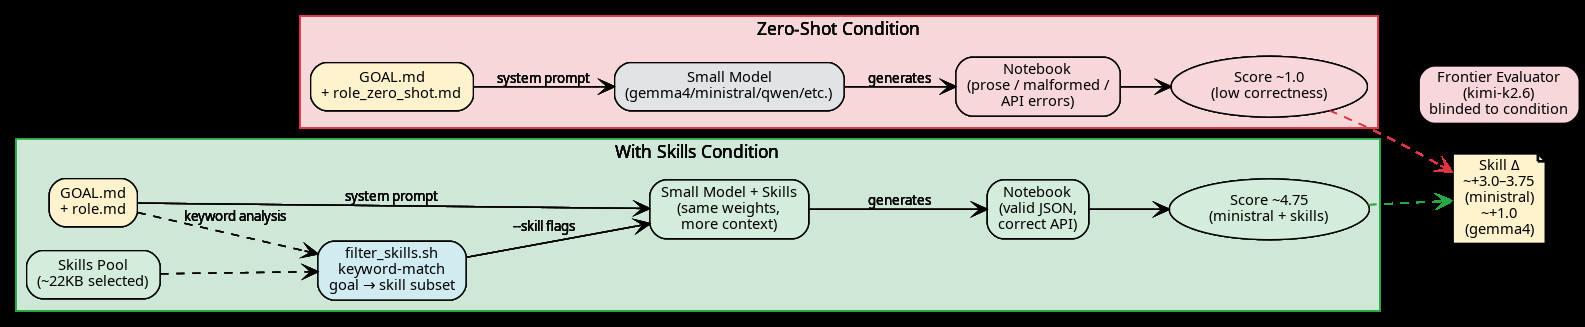
\includegraphics[width=\linewidth]{comparison_diagram.jpg}
    \end{column}
  \end{columns}
\end{frame}

\end{document}
